\documentclass[paper=a4, fontsize=12pt]{article} % A4 paper and 11pt font size
\usepackage[T1]{fontenc} % Use 8-bit encoding that has 256 glyphs
\usepackage[english]{babel} % English language/hyphenation
\usepackage{amsmath,amsfonts,amsthm} % Math packages
\usepackage{a4wide}
\usepackage{float}
\usepackage{longtable}
\usepackage{hyperref}
\usepackage{listings}
\usepackage{makecell}
\usepackage{graphicx}
\usepackage[table]{xcolor}
\usepackage[numbered, framed]{mcode}  % To load matlab code
\lstset{deletestring=[b]{"}}

\usepackage{fancyhdr} % Custom headers and footers
\pagestyle{fancyplain} % Makes all pages in the document conform to the custom headers and footers
\setlength\parindent{0pt}
\fancyhead[L]{SF3565, Project 3, November 2016}
\fancyhead[R]{H{\"a}ggmark, Karlsson} % Empty left footer
\fancyfoot[C]{Program construction in C++ for Scientific Computing} % Empty center footer
\fancyfoot[R]{\thepage} % Page numbering for right footer

\title{Program construction in C++ for Scientific Computing \\ Teacher: Michael Hanke}

\author{Ilian H{\"a}ggmark \\ mail \href{mailto:ilianh@kth.se}{ilianh@kth.se}
  \and Andreas Karlsson \\ mail \href{mailto:andreas.a.karlsson@ki.se}{andreas.a.karlsson@ki.se} }
\date{\normalsize\today} % Today's date or a custom date

\begin{document}

\maketitle % Print the title

\section*{Project 3}
\subsection*{Task 1 - Abstract Class}

The class \texttt{Curvebase} is created to hold basic functionality for curves, but not the curves themselves. The class has therefore the functions \texttt{x} and \texttt{y} that call the derived classes that contain the specific curve information. The grid generation for which the class will be used should not know about specifics either so the \texttt{Curvebase} is a kind of interfaces that convert a normalized position on a curve (zero to one) to the actual position that the grid point generation requires. The functions \texttt{x} and \texttt{y} will thus take the normalized arc length parameter $s$ and return \texttt{xp}$(p)$ and \texttt{yp}$(p)$ respectively. The functions \texttt{xp} and \texttt{yp} are pure virtual function (i.e. must be implemented in the derived class) that return $x$ and $y$ values given $p$ which is the actual position on the curved. Before calling \texttt{xp} and \texttt{yp} Curvebase must calculate $p$ from $s$. This is done by solving the equation

$$ \texttt{fp}(p) = \ell(p)- s\cdot  \ell(b) = 0 $$

where

$$ \ell (p) = \int_a^p \sqrt{\texttt{dxp}(q)^2+\texttt{dyp}(q)^2} \textrm{d}q $$

$a$ and $b$ are the lower and upper bounds of the curve and \texttt{dxp} and \texttt{dyp} are the derivatives of \texttt{xp} and \texttt{yp}. $\ell (p)$ gives the length between $a$ and $p$. $\ell (b)$ gives thus the total length of the curve. Newton's equation is used to solve the first equation.\\

The function \texttt{fp()} in \texttt{Curvebase} is used to calculate $p$ with Newton's methods. This is performed many times during the grid generation and the efficiency should be considered. \texttt{fp()} needs the total length of the curve, $\ell (b)$. This can be done by calling integrate. Doing this every time \texttt{fp()} is called is however not smart since the length of a curve is constant. We therefore want to create a variable in the \texttt{Curvebase} that contains the length. \texttt{Curvebase} is however an abstract class and does no know anything about the curve. We solve this by declaring a length variable in \texttt{Curvebase} and then initializing the variable in the constructor of the derived class. Setting length as a variable gives an decrease in computational time by a factor $\sim 2.5$.\\



\subsection*{Task 2 - Curve Generation}

The derived curve objects are quite simple since most of the machinery lies in the abstract class. The derived object mainly holds two important things: the limits of the curve ($a$ and $b$) and the description of the curve in terms of the functions \texttt{xp}, \texttt{yp}, \texttt{dxp}, and \texttt{dyp}. These functions simply contain the mathematical description of the curves.

\subsection*{Task 3 - Domain Class}

The Domain class takes four (4) curve objects and generates the grid points with the function \texttt{generate\_grid()}.\\

The most important part in terms of efficiency for this project is the nested loop that calculates grid points inside the \texttt{generate\_grid()} function. The expression used to calculate the $x$ coordinate (for the $y$-term $x$ is simply exchanged for $y$) from the normalized arc length parameter $s$ is

\begin{align*}
x[j+i*(m\_+1)]  &= \varphi_1(ih_1)\cdot \textrm{sides}[3]-\!\!>\texttt{x}(jh_2) \\
	&+ \varphi_2(ih_1)\cdot \textrm{sides}[1]-\!\!>\texttt{x}(jh_2) \\
	&+ \varphi_1(ih_2)\cdot \textrm{sides}[0]-\!\!>\texttt{x}(ih_1) \\
	&+ \varphi_2(jh_2)\cdot \textrm{sides}[2]-\!\!>\texttt{x}(ih_1) \\
	&- \varphi_1(ih_1) \varphi_1(jh_2) \cdot  \textrm{sides}[0]-\!\!>\texttt{x}(0) \\
	&- \varphi_2(ih_1) \varphi_1(jh_2) \cdot  \textrm{sides}[1]-\!\!>\texttt{x}(0) \\
	&- \varphi_1(ih_1) \varphi_2(jh_2) \cdot  \textrm{sides}[3]-\!\!>\texttt{x}(1) \\
	&- \varphi_2(ih_1) \varphi_2(jh_2) \cdot  \textrm{sides}[2]-\!\!>\texttt{x}(1)
\end{align*}

where $s$ is given by $ih_1$ and $jh_2$ depending on the direction. The four last terms are corner correction terms. Calculating this expression $(m\_+1)(n\_+1)$ times is very inefficient since the calling and calculation of the \texttt{x}-function of a side is computationally heavy. We can however reduce the number of calls. The $\varphi$-functions are very small and can be left as they are (inlining might give a little improvement but the compiler will probably perform inlining even without an explicit ``inline declaration''). We should however lift out the parts that contain the calls to sides.\texttt{x}(). We note that the ``sides'' part of the four corner terms does not depend on $i$ and $j$. It is thus extremely inefficient to recalculate them for every loop iteration. We can simply calculate them once before the loop starts. We also note that the first four lines are calculated $(m\_+1)(n\_+1)$ times even though $(m\_+1)$ times or $(n\_+1)$ times would be enough. We do this by calculating the first two lines in one loop and storing them in a vector, then doing the same thing for the 3rd and 4th line. The nested loop that finally puts everything together will thus not contain one call to the heavy \texttt{x}-function. This gives totally a decrease in computational time by a factor $\sim 2n\_ $ or $2m\_ $ depending how you write the nested loop. After the improvements generating one million grid points took e.g. $2.5$ seconds on an average Intel core duo processor (from 2008).  \\

\subsection*{Task 4 - Data Exportation}

A public function in the Domain class, \texttt{save2file}, writes the grid points to a binary file. The function takes the file name of the output file as an argument. The vectors \texttt{x\_} and \texttt{y\_} are concatenated before they are saved with the code given in the task. The produced file can then be read and visualized, as can be seen in Figure \ref{fig:grid}, using the \textsc{Matlab} code below.

\begin{lstlisting}
  fid = fopen('outfile.bin','r'); % open file
  c = fread(fid,'double');        % load file content to vector c

  x = c(1:length(c)/2);           % first half of c is x values
  y = c(length(c)/2+1:end);       % second half of c is y values

  plot(x,y,'.')                   % plot the x,y points

\end{lstlisting}
%  \label{lst:matlab}.
\begin{figure}[H]
  \centering
  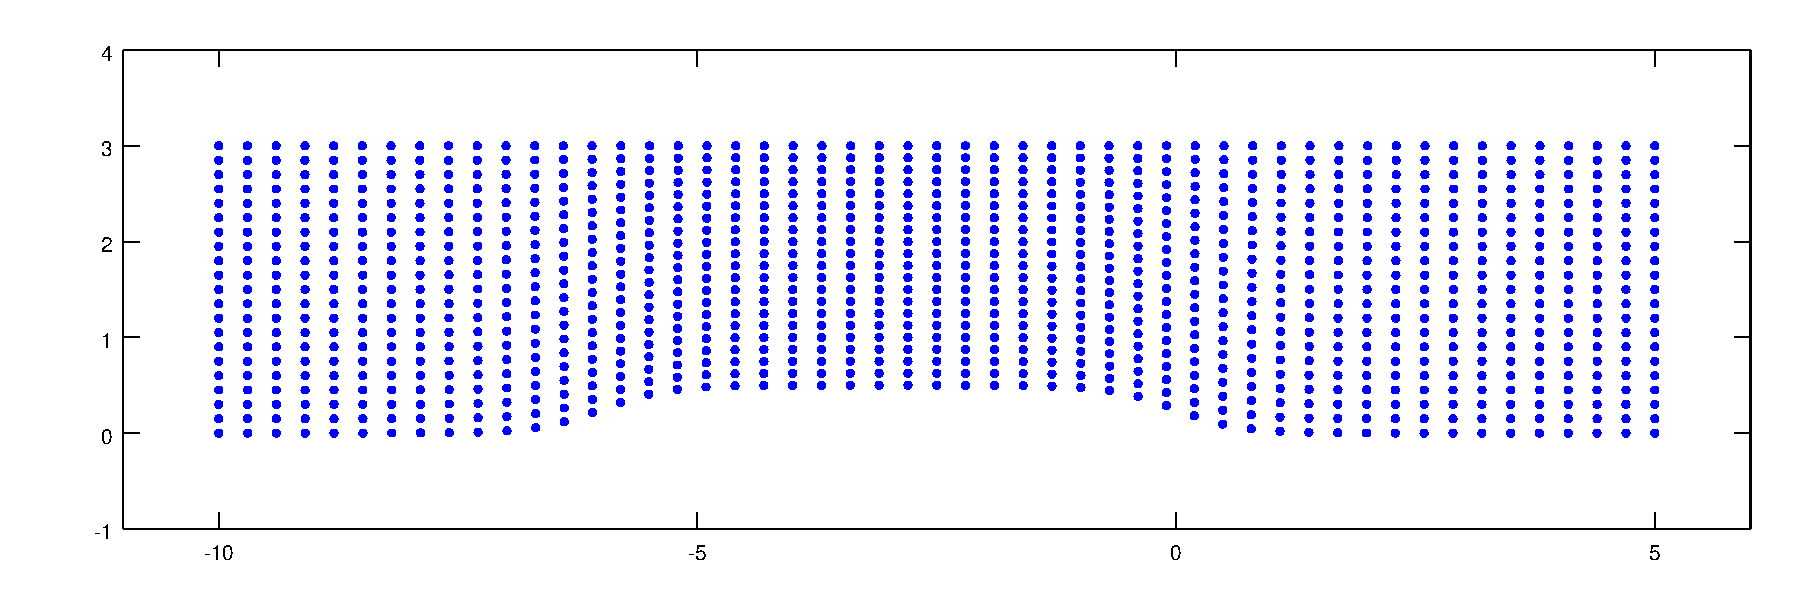
\includegraphics[width=\textwidth]{task4.pdf}
  \caption{\small $50\times 20$ Grid produced by the \texttt{generate\_grid()} method and plotted with \textsc{Matlab.}\label{fig:grid}}
\end{figure}

\subsection*{Task 5 - Grid stretching}


By adding an (optional) boolean argument in the \texttt{generate\_grid()} method the user can choose to stretch the grid. The expression given in task 5 was modified to

$$ ss = \frac{\exp(1.5s)-1}{\exp(1.5)-1}$$

and applied to $j*h_2$ in the calls to the functions \texttt{x} and \texttt{y} in \texttt{Curvebase}. This stretches the grid in the vertical direction, while still not changing the boundaries (as desired) as can be seen in Figure \ref{fig:stretched}. By changing the size and the sign of constant found in the expression above (here 1.5) the degree of stretching and the direction of increasing point density (up or down) can be controlled.

\begin{figure}[H]
  \centering
  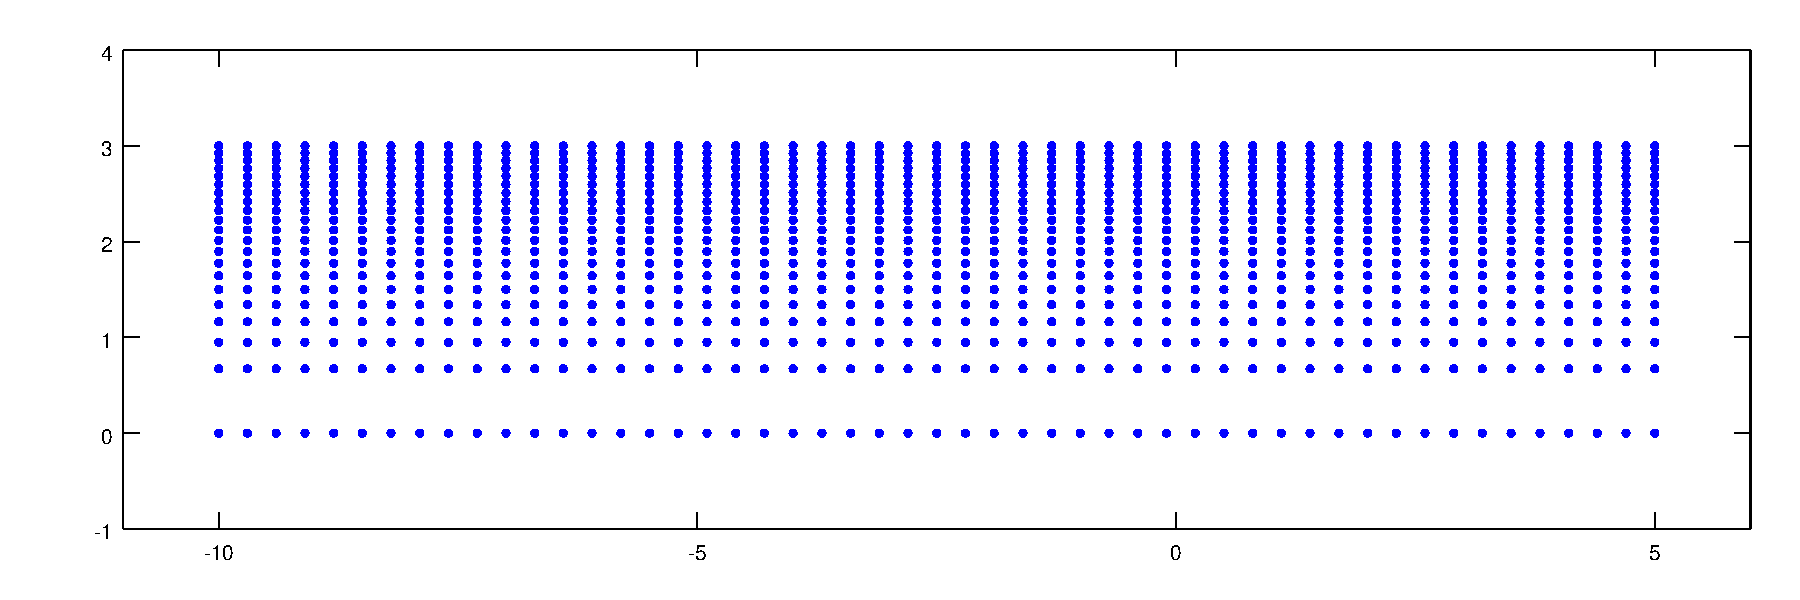
\includegraphics[width=\textwidth]{task5.pdf}
  \caption{\small A stretched grid ($50\times 20$) plotted with \textsc{Matlab.}\label{fig:stretched}}
\end{figure}



\end{document}
